\section{Three NO$_2$ interventions with charged acquisition}
The I2R proposal motivates layered HITRAN modeling, statistical ratiometric inversion and sensitivity analysis; it supplies no repeated receiver calibration records. We therefore distinguish physical inputs, mathematical error models and missing calibration evidence. A laboratory THz study illustrates why reference repeatability and frequency tuning require separate characterization~\cite{bjarnason2008}; its methyl-chloride apparatus does not calibrate our NO$_2$ receiver.

\subsection{Differencing and structured calibration}
Temporal subtraction gives
\[
y_1-y_0=D(\theta_1-\theta_0)+N(\beta_1-\beta_0)
+(b_1-b_0)+(n_1-n_0).
\]
Identical persistent instrumental error cancels. Independent per-reading error boxes of radius $\epsilon$ instead leave a box of radius $2\epsilon$. Concentration changes are the estimand; absolute concentration additionally needs a baseline estimate and its covariance. Independent readings with equal noise have doubled variance at equal per-reading dwell. At equal \emph{total} acquisition time, halving the budget of each reading gives four times the variance before extra retuning. We use $2\operatorname{conv}\{\pm b_s\}$ for atmospheric difference error, so the design does not assume atmospheric cancellation.

Spectral differencing alone is a coordinate change on the offset-free observation space. Propagating the full contrast covariance gives a NO$_2$ GLS variance ratio of 1.000000000005 relative to the original observations with an unknown offset. Treating shared-reference contrasts as independent would create a spurious gain.

For structured calibration write $b_{\rm cal}=S\gamma+u$, $|\gamma_k|\le1$ and $\|u\|_\infty\le\epsilon_r$. The exact support contribution is $\|S^Th\|_1+\epsilon_r\|h\|_1$. Our exploratory $S$ contains degree-zero, one and two Legendre modes on 260--400 GHz, each scaled by $(\epsilon-\epsilon_r)/3$. This set is a subset of the original radius-$\epsilon$ box. It represents stronger assumptions, not measured improvement in an instrument. The constant mode is already canceled by $N$. We retain $\epsilon=10^{-4}$ dB with residual zero or $10^{-5}$ dB, and implement a separate chronological reference-sweep characterization tool. No receiver recordings are available to run that characterization.

\subsection{New frequencies and jointly optimized dwell}
We evaluate a 0.25 GHz candidate grid together with all 71 prior band probes, directly recomputing the 24-layer Voigt spectra and all 54 design discrepancies. Retaining new probes with nominal SNR at least 5 dB at $-1$ dBm leaves 424 frequencies. All coefficients and scenario choices precede the new stress evaluation. With per-second noise coefficient $a_i$, eliminating continuous dwell under $\sum_i t_i=T_a$ gives
\begin{equation}
\min_{t_i\ge0,\,\sum t_i=T_a}\sum_i\frac{a_i h_i^2}{t_i}
=\frac{\big(\sum_i|h_i|\sqrt{a_i}\big)^2}{T_a},
\qquad t_i\propto|h_i|\sqrt{a_i}.
\end{equation}
The zero-weight terms use zero dwell in this relaxation. Combining its square root with atmospheric and calibration support functions yields a convex target-specific design. The NO$_2$ row cancels the other three gas responses and the original nuisance spectra; it does not guarantee simultaneous four-gas precision.

All primary comparisons use one active $-1$ dBm tone, 1 $\mu$s pilots, 10 or 100 s total charged acquisition and an assumed 1 ms retuning time. One or two sorted sweeps cost respectively $m-1$ or $2(m-1)$ retunings. We round to integer pilots, visit every retained frequency at least once, preserve the jointly optimized operator and recompute its achieved risk. The largest rounding increment in RMSE is 0.000338. Integer optimality is not claimed. Fixed-allocation reoptimization attempts with inaccurate solver status were rejected and archived. The final 30 configurations pass independent arithmetic and constraint checks.

\begin{figure*}[t]\centering
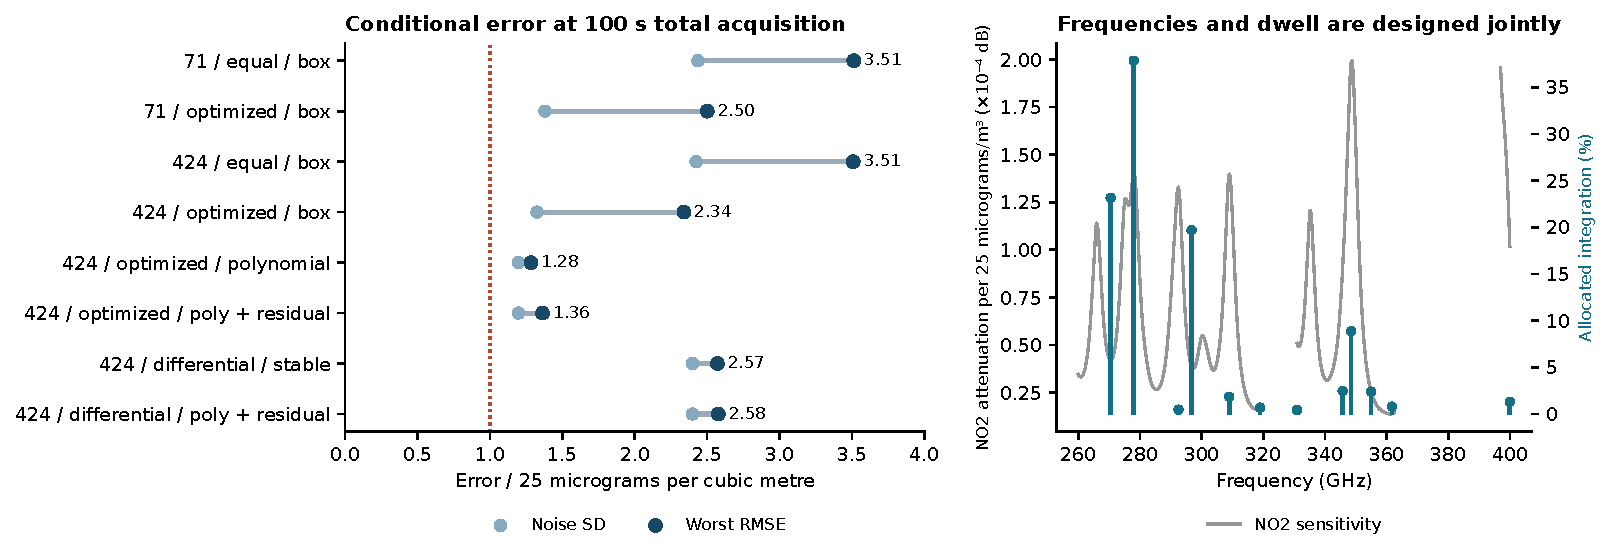
\includegraphics[width=.99\textwidth]{../results/no2_three_routes/report/no2_routes.pdf}
\caption{NO$_2$ design comparisons with explicit time and calibration assumptions. Left: one-spectrum absolute retrieval and two-spectrum change retrieval use the same total acquisition budget, but different estimands and error sets. Right: the mixed polynomial/residual design assigns time to both signal and control frequencies. All results use modeled attenuation and nominal coherent noise.}
\end{figure*}
\begin{table}[t]\centering\scriptsize
\caption{Worst design RMSE at 100 s charged acquisition, divided by 25 \ugm. The original box has radius $10^{-4}$ dB; the mixed absolute model retains $10^{-5}$ dB arbitrary residual.}
\begin{tabular}{lr}\toprule
Probes, allocation and error model & RMSE\\\midrule
71, equal, box & 3.513\\
71, optimized, box & 2.501\\
424, equal, box & 3.509\\
424, optimized, box & 2.340\\
424, polynomial & 1.283\\
424, polynomial + residual & 1.363\\
424, change, stable calibration & 2.571\\
424, change, polynomial + residual & 2.578\\
\bottomrule\end{tabular}
\end{table}

Most of the gain comes from dwell allocation: the coarse equal/optimized box errors are 3.513 and 2.501. Fine equal dwell gives 3.509, while fine optimized dwell gives 2.340. A separate rational dual check gives a noise-free box floor of 1.923285 on the 424 probes, compared with 2.055634 on the 71 probes. Both exceed one. The new frequencies improve this represented-model floor but do not eliminate it.

Under the declared pure polynomial error model the fine design reaches 1.283 at 100 s; retaining the arbitrary $10^{-5}$ dB residual gives 1.363. Holding each 100 s operator and its allocation proportions fixed, 181.798 and 248.809 s respectively suffice numerically to reach the unit design target, after charging integer pilots and retuning. These are constructive times for those particular designs, not minimum-time bounds. The latter case radiates 0.1973 J. Stable-calibration differential retrieval requires 3902.121 s for its frozen design and conservative atmospheric-difference envelope. Such long acquisitions additionally require unverified stationarity and geometry control. Narrowing the calibration set cannot be presented as evidence that this stability has been achieved.

\subsection{New modeled states and real meteorological changes}
We freeze all operators before evaluating 16 new assumed temperature/pressure/height states using real test-period concentrations and 24 same-station pairs separated by one recorded hour. Both endpoints lie after the existing validation cutoff. The pair experiment uses the recorded temperature, pressure and dew point, with the same assumed 1.5 km pollutant profile. It repeats a fixed 45-degree slant geometry; these are not synchronized satellite overpasses or measured radio data. Acquisition time excludes the hour between epochs and initial setup. The previously used public concentration records are not a new independent population sample.

At 100 s, the mixed structured fine design has worst RMSE 1.291 on the 16 new states under nominal covariance (1.306 with modeled state-dependent noise). On the hourly meteorological pairs, absolute atmospheric bias reaches 3.201, beyond the design envelope. Stable-calibration differencing reduces the corresponding worst change bias to 0.411, but its nominal noise SD rises to 2.399. Its worst pair RMSE is 2.434, versus 3.597 for the mixed structured absolute estimator; neither reaches one and their estimands differ.

Eleven of 24 weather pairs place at least one visited tone below the 5 dB design regime. Substituting the modeled weather-dependent covariance produces worst errors of 26.280 for mixed structured absolute retrieval and 47.243 for stable differential retrieval. These numbers are extrapolated diagnostics where the coherent approximation may fail, not validated performance predictions. The loss of the nominal SNR regime itself prevents claiming robust field retrieval. Measured spectral drift, realistic geometry and calibration across humidity changes remain necessary.
